\documentclass[../main.tex]{subfiles}

    \begin{document}
    \newpage

%%%%%%%%%%%%%%
    % Volet
    \vspace{15pt}
    %\needspace{20pt} % Réserve de l'espace
\section{Information et communication}

    % Block
\begin{block}[Sensibiliser]
    \linespread{0.9}\selectfont % Réduit l'interligne
    \emoji{compass} % Emoji
    \textit{\small{Améliorer l'accès à l'information et sensibiliser aux bénéfices de l'usage intermodal de la mobilité individuelle légère.}}
\end{block}

    \begin{multicols}{2}
    \raggedcolumns
    \small{
L’accessibilité et la lisibilité \gras{de l’information} sont des leviers stratégiques pour encourager l’usage intégré du vélo et de la micro-mobilité. \gras{Une signalétique} claire et homogène, associée à \gras{des plans} lisibles et accessibles, est essentielle pour guider les usagers.
    \\\\
Par ailleurs, \gras{une campagne de sensibilisation} visant à mieux faire connaître les avantages pratiques, économiques et environnementaux de l’intermodalité cyclable peut jouer un rôle clé dans \gras{l’évolution des comportements}, comme l’a mis en évidence notre étude en analysant les déterminants des choix modaux dans la région.
    \\\\
Informer efficacement les usagers sur les services disponibles, les connexions possibles et les outils facilitant l'intermodalité, notamment à l'aide \gras{d'applications numériques} et \gras{de dispositifs} en gare, contribuerait à lever les freins à l’usage et à ancrer durablement ces pratiques dans les habitudes de mobilité.
    }
    \end{multicols}

\begin{figure}[h!]\vspace*{10pt}
    \captionsetup{labelformat=empty, labelsep=none} % Supprime la numérotation
        %\caption{\textbf{Diagramme.} Fleur schématique synthétisant les dix volets pour aménager des quartiers de gare piétons et cyclables favorables à un système urbain et de mobilité soutenables}
        \label{raisons-adoption}
        \centerline{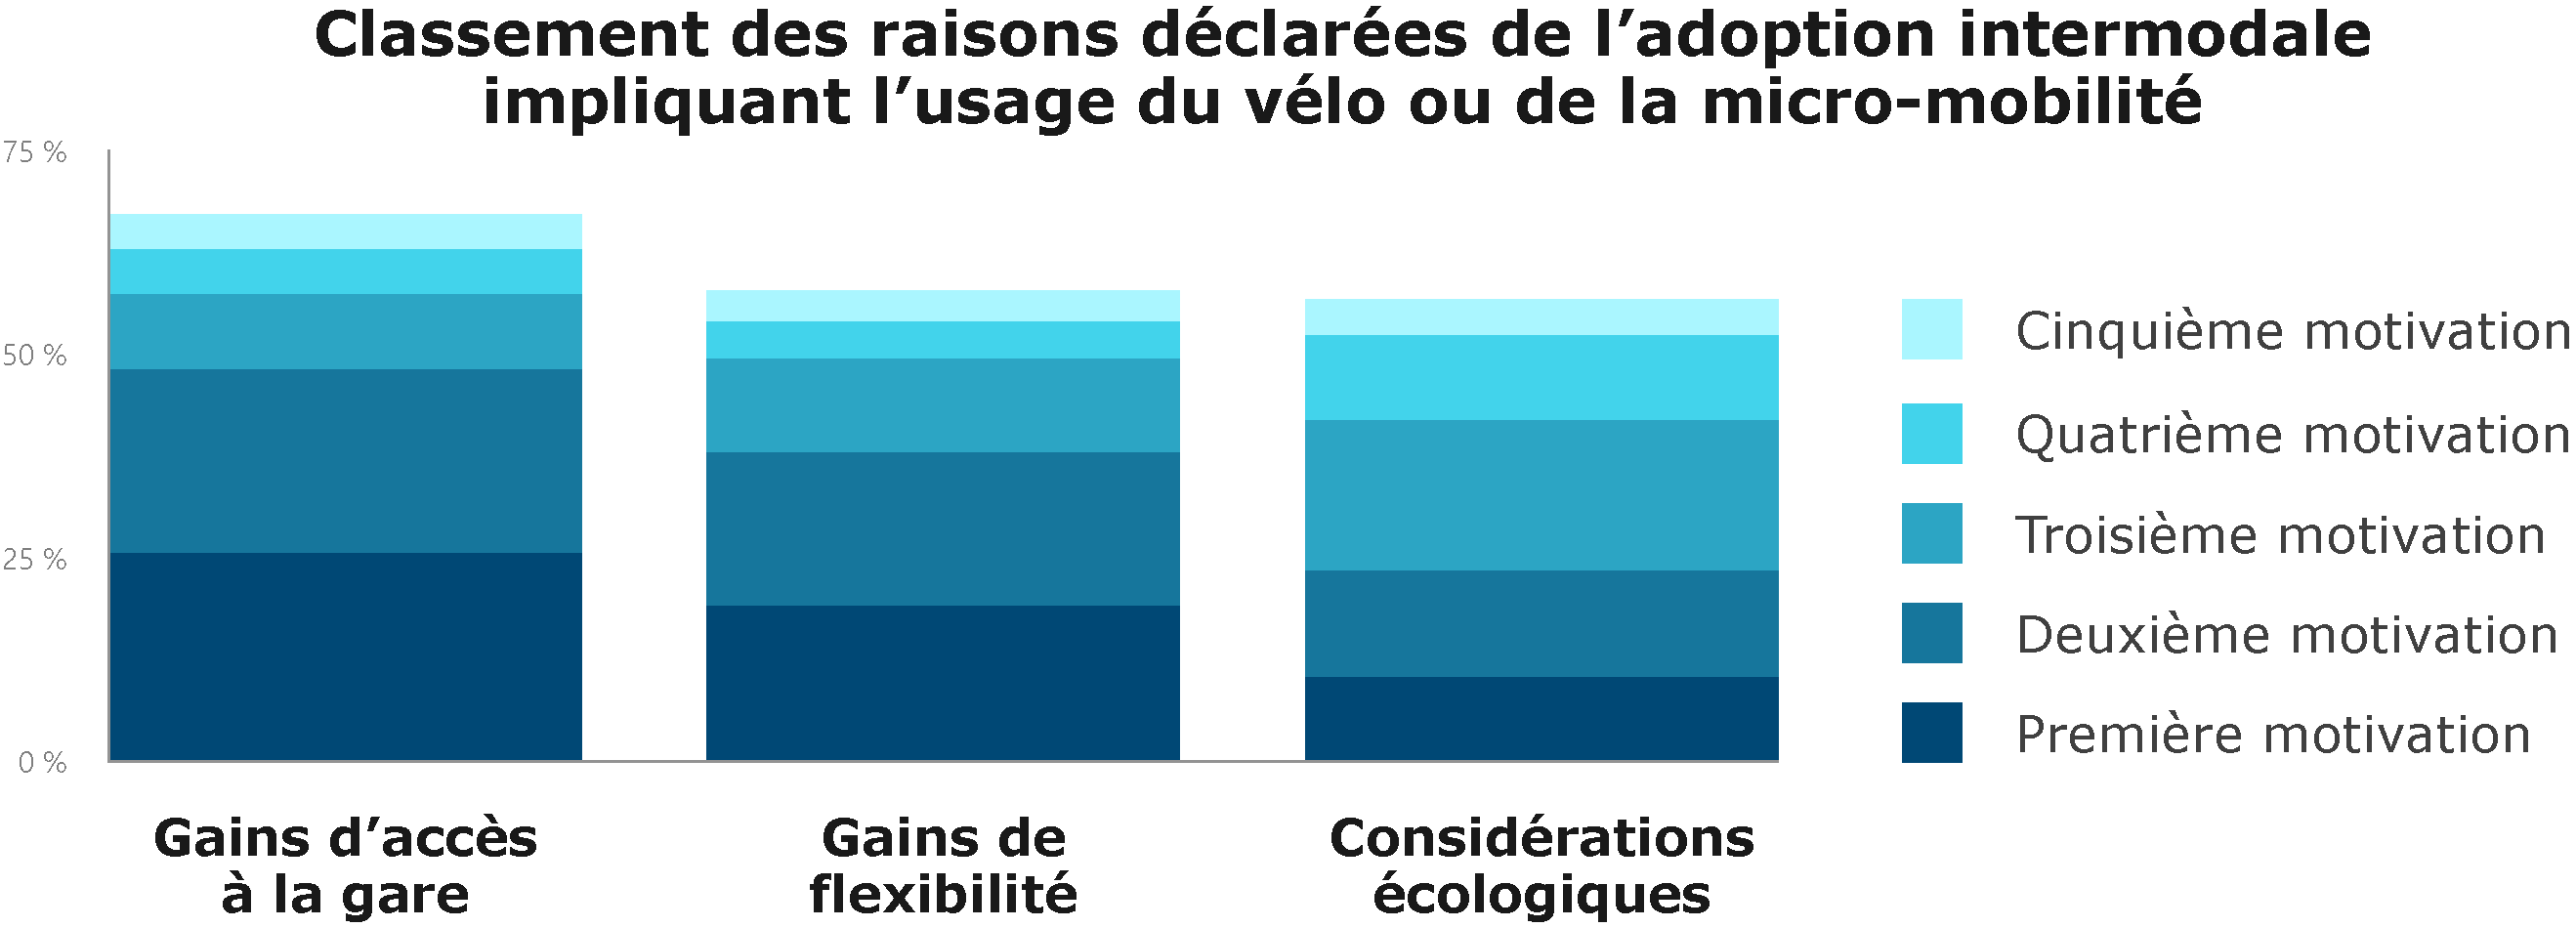
\includegraphics[width=1\columnwidth]{figures/policy-brief-raisons-adoption.pdf}}
        \vspace{3pt}
        \begin{flushright}\scriptsize{
        Auteur~: \textcolor{UGEblue}{Dylan Moinse (2025)}
        }\end{flushright}
    \end{figure}

    \end{document}